\documentclass[11pt,a4paper]{article}

\usepackage[margin=24mm]{geometry}
\usepackage{fontspec}
\usepackage{libertinus}
\usepackage{microtype}
\usepackage{amsmath,amsthm,mathtools}
\usepackage{booktabs,tabularx,longtable,array,multirow}
\usepackage{graphicx}
\usepackage{tikz}
\usetikzlibrary{arrows.meta,positioning,shapes.geometric,fit}
\usepackage{caption}
\usepackage{subcaption}
\usepackage{enumitem}
\usepackage{siunitx}
\usepackage{xcolor}
\usepackage{xurl}
\usepackage{hyperref}
\usepackage[nameinlink,noabbrev]{cleveref}
\usepackage[backend=biber,style=authoryear,maxcitenames=2,maxbibnames=99,doi=false,isbn=false]{biblatex}
\addbibresource{references.bib}

\definecolor{navy}{HTML}{17365D}
\definecolor{blue}{HTML}{2F6FD0}
\definecolor{softblue}{HTML}{EAF1FB}
\definecolor{softgray}{HTML}{F4F5F7}
\definecolor{darkgray}{HTML}{3F4752}
\hypersetup{colorlinks=true,linkcolor=navy,citecolor=navy,urlcolor=blue,pdfauthor={Tivdzua Lubem Noah},pdftitle={Risk-Controlled Decision-Value Acquisition for Runtime Safety Monitor Fusion}}

\newtheorem{proposition}{Proposition}
\newtheorem{example}{Counterexample}
\newcommand{\code}[1]{\texttt{#1}}
\newcommand{\pass}{\textbf{Pass}}
\newcommand{\nogo}{\textbf{No-go}}
\newcommand{\R}{\mathbb{R}}
\newcolumntype{Y}{>{\raggedright\arraybackslash}X}
\setlist{nosep,leftmargin=*}
\sisetup{round-mode=places,round-precision=3,detect-all}

\title{\textbf{Risk-Controlled Decision-Value Acquisition for Runtime Safety Monitor Fusion}}
\author{Tivdzua Lubem Noah\\\small Trustworthy AI Course Project}
\date{31 July 2026}

\begin{document}

\pagenumbering{arabic}
\maketitle
\thispagestyle{plain}

\begin{abstract}
Runtime safety systems often combine inexpensive filters with a stronger but slower monitor. A common routing rule sends uncertain examples to the expensive monitor. That rule is not generally optimal: acquisition is useful only when the optional monitor is expected to improve the downstream decision enough to justify its cost. This study formalizes that distinction through conditional decision value, constructs a counterexample in which cheap uncertainty is identical but optional-monitor quality differs, and verifies the mechanism in a two-context Gaussian simulation.

The real-data analysis uses 1,687 development examples from an audited 2,159-example prompt-response dataset. Two optional acquisitions are considered: compact moderation after a deterministic rule filter, and Qwen3Guard after the rule and compact monitor. Realized value targets are generated with nested cross-fitting. Six prespecified feature families are evaluated using outer-fold predictions, exact matched acquisition counts, and a paired 2,000-repetition bootstrap. Qwen provides substantial complementary value: always acquiring it reduces cross-fitted decision loss from 0.1749 to 0.0676. The primary learned-value policy has a positive integrated advantage of 0.00482 over ordinary uncertainty, but its 95\% confidence interval is $[-0.00170,\,0.01149]$. The prespecified predictability condition therefore does not pass.

A separate common-risk frontier does pass empirically on development data. The lowest-cost passing point acquires Qwen for 9.78\% of examples, reaches recall 0.3368 at FPR 0.0287, and exceeds uncertainty and the 97.5th-percentile random baseline under the same incremental-cost ceiling. Because the predictability gate failed, the overall milestone remains no-go. The result supports decision value as the correct acquisition target, while showing that the available legitimate pre-acquisition features do not establish a statistically reliable improvement over uncertainty on this dataset.
\end{abstract}

\noindent\textbf{Keywords:} runtime safety monitoring; value of information; selective acquisition; risk control; cross-fitting; trustworthy AI.
\vspace{0.8em}

\section{Introduction}

Runtime moderation has a natural cost hierarchy. A deterministic filter can run in approximately one millisecond, a compact classifier takes tens of milliseconds, and a generative safety judge may take more than a second. Calling every monitor on every interaction is costly, but skipping the stronger monitor can alter the final safety decision. The central question is therefore not whether an example appears harmful or uncertain in isolation. It is whether obtaining a particular monitor output is expected to improve the downstream decision enough to justify its cost.

The project began with a threshold-based selective router. That implementation reduced mean latency by 24.34\% on a 128-example Tesla T4 benchmark, but the prespecified 5\% false-positive requirement did not hold reliably under the audited source and attack-family stress tests. The original result was consequently retained as a measurement-validity finding rather than a deployment claim. The subsequent work did not continue optimizing the low/high routing thresholds. It followed a narrower question: can acquisition be based on monitor-specific decision value rather than ordinary uncertainty?

This report combines the complete project record. The initial audited monitor-fusion pipeline is retained as context; the main analysis is the professor-directed decision-value pivot. The contributions are:

\begin{enumerate}
  \item a conditional decision-value formulation and optimal two-monitor acquisition rule;
  \item a counterexample showing that identical cheap uncertainty can coexist with different optional-monitor value;
  \item a controlled two-context Gaussian experiment comparing random, uncertainty, oracle-value, and learned-value acquisition at identical rates;
  \item leakage-controlled, nested cross-fitted targets for two real optional-monitor setups;
  \item a six-family value-predictability diagnostic using complete-text frozen embeddings and legitimate runtime metadata;
  \item matched-budget and common-risk safety-cost comparisons with measured inference costs; and
  \item a prespecified no-go interpretation that leaves excluded evaluation partitions unused.
\end{enumerate}

The study does not introduce a validated new routing method. It does not establish robustness to changing attack distributions, detection of correlated monitor failures, or deployment readiness.

\section{Related work and project context}

The dataset combines examples from JailbreakBench, XSTest, and WildGuardTest. JailbreakBench standardizes adversarial prompting and jailbreak evaluation \parencite{chao2024jailbreakbench}. XSTest contains safe prompts designed to expose exaggerated safety behavior \parencite{rottger2024xstest}. WildGuard provides prompt-harmfulness, response-harmfulness, and refusal annotations for safety moderation \parencite{han2024wildguard}. These sources serve different purposes; their combination increases coverage but does not make the resulting sample representative of deployment traffic.

The monitor stack contains a deterministic lexical rule filter, the KoalaAI text-moderation classifier \parencite{koala2023moderation}, and Qwen3Guard-Gen-4B \parencite{zhao2025qwen3guard}. The decision-value analysis also uses the 384-dimensional all-MiniLM-L6-v2 representation \parencite{wang2020minilm,reimers2021allminilm}. All learned monitors and the embedding model are pinned to recorded revisions.

Selective classification usually trades coverage for predictive risk \parencite{elyaniv2010selective}. Cost-sensitive feature acquisition instead asks whether a missing feature is worth purchasing given its expected reduction in decision loss \parencite{bilgic2014voila}. The present study treats a safety monitor as an optional feature with nontrivial latency. Learn-then-Test risk control is relevant to the earlier in-distribution calibration analysis \parencite{angelopoulos2025ltt}; its guarantees are not interpreted as automatically transferring across source or attack-family shifts.

\section{Problem formulation}

\subsection{Prediction target and monitor sequence}

Each observation is a prompt-response pair $X=(P,R)$. The label $Y=1$ means that the response should be intercepted because, in the context of the prompt, it materially provides, facilitates, endorses, or contains disallowed harmful content. Benign answers, safe refusals, and safe redirections have label $Y=0$.

The sequential system is shown in \cref{fig:pipeline}. The real-data pivot evaluates two acquisition stages separately:

\begin{enumerate}
  \item \textbf{compact after rule}: the rule score is available before deciding whether to obtain the compact score;
  \item \textbf{Qwen after rule and compact}: rule and compact outputs are available before deciding whether to obtain the Qwen prompt-response score.
\end{enumerate}

\begin{figure}[htbp]
\centering
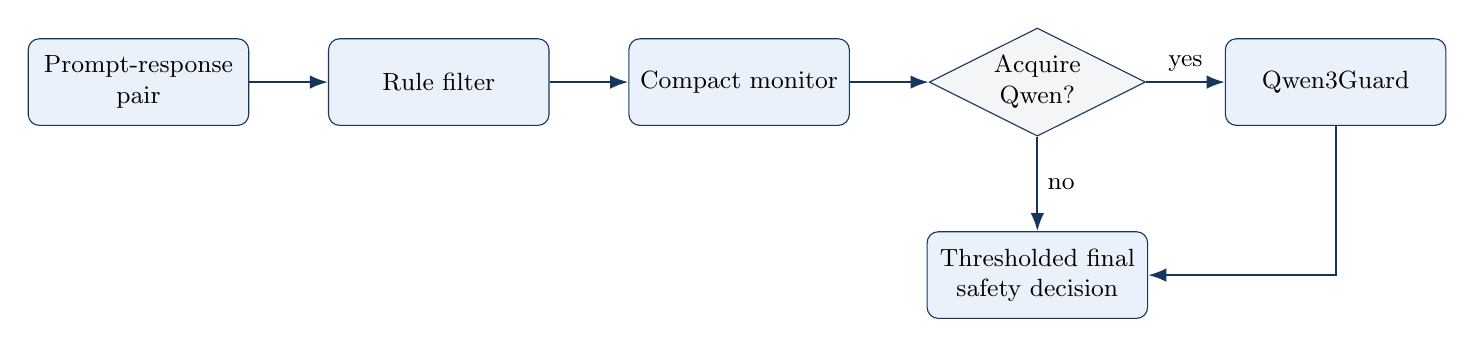
\begin{tikzpicture}[node distance=8mm and 10mm, every node/.style={font=\small}, box/.style={draw=navy,rounded corners,fill=softblue,minimum width=28mm,minimum height=11mm,align=center}, decision/.style={diamond,draw=navy,fill=softgray,aspect=2,align=center,inner sep=1.5pt}, arr/.style={-{Latex[length=2.3mm]},thick,draw=navy}]
\node[box] (input) {Prompt-response\\pair};
\node[box,right=of input] (rule) {Rule filter};
\node[box,right=of rule] (compact) {Compact monitor};
\node[decision,right=of compact] (route) {Acquire\\Qwen?};
\node[box,right=of route] (qwen) {Qwen3Guard};
\node[box,below=12mm of route] (final) {Thresholded final\\safety decision};
\draw[arr] (input) -- (rule);
\draw[arr] (rule) -- (compact);
\draw[arr] (compact) -- (route);
\draw[arr] (route) -- node[above]{yes} (qwen);
\draw[arr] (qwen) |- (final);
\draw[arr] (route) -- node[right]{no} (final);
\end{tikzpicture}
\caption{Sequential monitor acquisition evaluated in the primary real-data setup. Optional-monitor outputs are used to define realized value but are prohibited as pre-acquisition predictors.}
\label{fig:pipeline}
\end{figure}

\subsection{Decision value}

Let $H$ denote all legitimate information available before an optional monitor is acquired, and let $Z$ be its output. For downstream action $a\in\mathcal{A}$ and loss $\ell(a,Y)$, define the conditional Bayes risk without acquisition as
\begin{equation}
  r(h)=\inf_{a\in\mathcal{A}}\mathbb{E}[\ell(a,Y)\mid H=h].
\end{equation}
After observing $Z=z$,
\begin{equation}
  r(h,z)=\inf_{a\in\mathcal{A}}\mathbb{E}[\ell(a,Y)\mid H=h,Z=z].
\end{equation}
For acquisition cost $c(h)\ge 0$, the conditional value before cost is
\begin{equation}
  \Delta(h)=r(h)-\mathbb{E}[r(h,Z)\mid H=h].
  \label{eq:value}
\end{equation}

\begin{proposition}[Optimal two-monitor acquisition]
For a fixed cheap-information state $h$, acquiring the optional monitor is strictly optimal if and only if
\begin{equation}
  \Delta(h)>c(h).
\end{equation}
Equality makes acquisition and non-acquisition conditionally equivalent.
\end{proposition}

\begin{proof}
Skipping has conditional risk $R_{\mathrm{skip}}(h)=r(h)$. Acquisition pays the cost and then optimizes after observing $Z$, giving
$R_{\mathrm{acquire}}(h)=c(h)+\mathbb{E}[r(h,Z)\mid H=h]$.
Acquisition is preferred exactly when $R_{\mathrm{acquire}}(h)<R_{\mathrm{skip}}(h)$, which rearranges to \cref{eq:value} exceeding $c(h)$.
\end{proof}

Because an action rule may ignore $Z$, expected post-acquisition Bayes risk cannot exceed $r(h)$, so $\Delta(h)\ge0$. Nonnegative value alone is insufficient; it must exceed acquisition cost.

\subsection{Why uncertainty is not enough}

Consider binary $Y$ and zero-one loss in two equally likely contexts $A$ and $B$. In both contexts, the cheap posterior is $\Pr(Y=1\mid H)=1/2$, so cheap uncertainty and Bayes risk are identical. In context $A$, the optional monitor is 90\% accurate, reducing Bayes risk from 0.5 to 0.1 and giving $\Delta(h_A)=0.4$. In context $B$, the monitor is independent of $Y$, leaving risk at 0.5 and giving $\Delta(h_B)=0$.

At 50\% acquisition, a value policy acquires all context-$A$ examples and no context-$B$ examples. Its decision loss is 0.3. An uncertainty policy cannot distinguish contexts and, under context-independent tie-breaking, acquires half of each; its loss is 0.4. Both have the same acquisition cost, but the uncertainty policy has 0.1 higher decision loss. The distinction is monitor-specific: uncertainty concerns the current prediction, whereas decision value concerns the expected improvement from a particular acquisition.

\section{Data, monitors, and measurement controls}

\subsection{Dataset and labels}

The audited dataset contains 2,159 prompt-response pairs: 200 JailbreakBench examples, 250 XSTest examples, and 1,709 WildGuardTest examples. The final labels contain 403 positives and 1,756 negatives. Two hundred rows were manually reviewed, a focused second review covered 40 difficult cases, and 19 labels were corrected. The review was conducted by one author; it is not a multi-rater annotation study.

The decision-value diagnostic uses only \code{policy\_train}, \code{policy\_selection}, and \code{calibration}: 1,687 rows with 291 positives and 1,396 negatives. The 422-row \code{final\_test} split and 50-row \code{held\_out\_shift} split were excluded from feature design, model fitting, threshold selection, and milestone decisions.

\begin{table}[htbp]
\centering
\caption{Data scope used in the completed project.}
\label{tab:data}
\begin{tabularx}{\textwidth}{@{}lrrY@{}}
\toprule
Partition or source & Examples & Positives & Role \\
\midrule
JailbreakBench & 200 & -- & Adversarial source component \\
XSTest & 250 & -- & Safe over-refusal probes \\
WildGuardTest & 1,709 & -- & Mixed response-safety examples \\
\midrule
Audited unified dataset & 2,159 & 403 & Full repository dataset \\
Development pool & 1,687 & 291 & All decision-value fitting and evaluation \\
Excluded final test & 422 & -- & Not used after the pivot \\
Excluded held-out shift & 50 & -- & Not used after the pivot \\
\bottomrule
\end{tabularx}
\end{table}

\subsection{Monitor and representation costs}

\Cref{tab:components} lists the measured components used in cost accounting. The final GPU timing benchmark used a Tesla T4, batch size 1, and 128 deterministic examples. The complete-text embedding was measured separately on CPU. The rule-plus-compact base cost is common to the primary learned, uncertainty, and random policies and is excluded from the incremental frontier; Qwen cost is multiplied by acquisition rate. The learned policy additionally pays the embedding and value-inference overhead on every example.

\begin{table}[htbp]
\centering
\caption{Frozen monitor and representation components.}
\label{tab:components}
\begin{tabularx}{\textwidth}{@{}lYrr@{}}
\toprule
Component & Implementation & Mean runtime (ms) & Role \\
\midrule
Rule filter & Deterministic weighted lexical rules & 1.271 & Always available \\
Compact monitor & KoalaAI/Text-Moderation, pinned revision & 45.657 & Cheap learned monitor \\
Qwen monitor & Qwen3Guard-Gen-4B, pinned revision & 1,597.561 & Optional expensive monitor \\
Frozen embedding & all-MiniLM-L6-v2, complete-text chunking & 159.468 & Learned-value predictor \\
PCA + value inference & 32-D PCA and gradient-boosting prediction & 0.029 & Learned-value predictor \\
\bottomrule
\end{tabularx}
\end{table}

\begin{figure}[htbp]
\centering
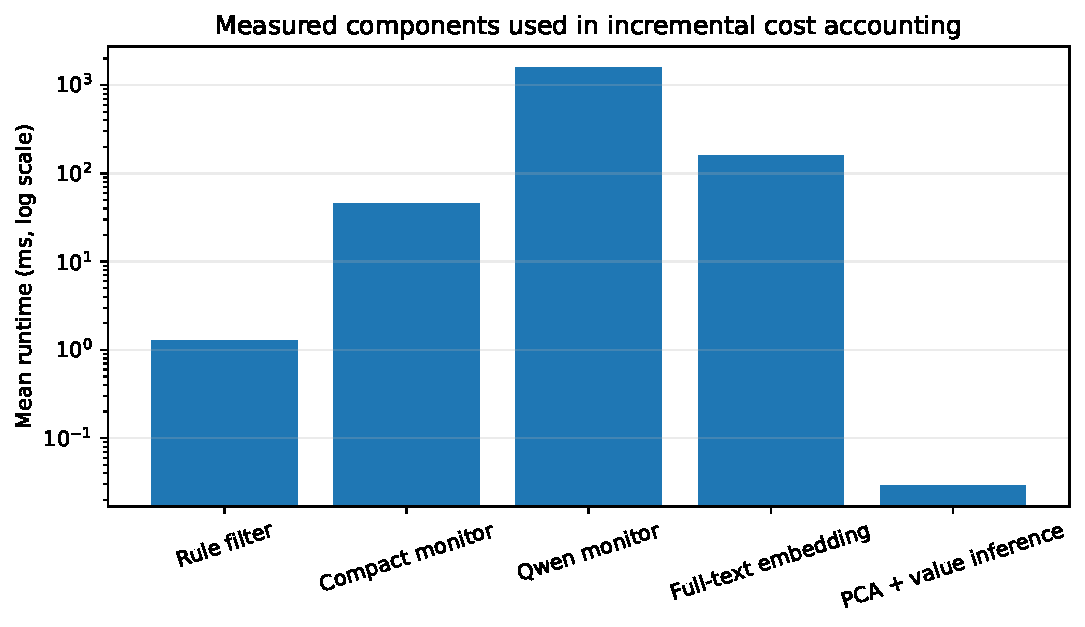
\includegraphics[width=0.78\textwidth]{figures/runtime_components.pdf}
\caption{Runtime components on a logarithmic scale. Hardware differs between the GPU monitor timing and CPU embedding/inference timing; values are used only in the documented incremental-cost calculation.}
\label{fig:runtime}
\end{figure}

\subsection{Complete-text embedding requirement}

The frozen representation uses \code{sentence-transformers/all-MiniLM-L6-v2}, resolved revision \code{1110a243...}. Prompt and response are placed in a fixed template, tokenized without truncation, divided into deterministic non-overlapping chunks, pooled with content-token-count weights, and L2-normalized. The artifact contains 1,687 vectors of dimension 384. It covers all 699,243 content tokens, has minimum per-example coverage 1.0, and records zero truncated examples. PCA is fitted only within the relevant training partition.

\section{Experimental design}

\subsection{Cross-fitted downstream decisions}

For each optional monitor and development example, realized decision value is
\begin{equation}
V_i=L(Y_i,\widehat a_{\mathrm{base},i})-L(Y_i,\widehat a_{\mathrm{augmented},i}).
\end{equation}
With zero-one loss, $V_i=1$ when acquisition corrects a decision, $V_i=0$ when loss is unchanged, and $V_i=-1$ when acquisition worsens it.

Five outer \code{StratifiedGroupKFold} partitions provide unseen development evaluation. Within each current outer-training partition, four inner folds create out-of-fold base and augmented scores and select decision thresholds at empirical FPR 0.05. The current value-estimator evaluation fold is excluded before these training targets are generated. The nested artifact contains 13,496 rows; each example/setup appears in four outer-training partitions, and the recorded outer-evaluation leakage count is zero.

\subsection{Predictor families}

Six families were fixed before fitting the value estimator:

\begin{enumerate}
  \item cheap monitor features;
  \item frozen prompt-response embedding;
  \item legitimate runtime metadata;
  \item cheap features plus metadata;
  \item cheap features plus embedding;
  \item all features.
\end{enumerate}

The primary comparison is Qwen after rule and compact with \code{all\_features}. Dataset source, attack family, split identity, labels, audit fields, and optional-monitor outputs are prohibited predictors. The estimator is \code{HistGradientBoostingRegressor}; three prespecified hyperparameter configurations are selected by inner-validation mean squared error. For embedding families, 32-component PCA is fitted separately inside each estimator inner-training split and then refitted on the complete current outer-training partition for its outer-fold prediction.

\subsection{Matched budgets and inferential criterion}

Random acquisition, ordinary uncertainty, learned decision value, and an oracle realized-value diagnostic are evaluated at exact within-fold counts corresponding to budgets of 0, 5, 10, 20, 30, 40, 50, 60, 75, and 100\%. Ties are resolved by a deterministic hash of \code{example\_id}. The primary predictability estimand is the trapezoidal integrated matched-budget decision-loss-reduction advantage of learned value over uncertainty. A paired bootstrap over development examples with 2,000 repetitions gives the 95\% confidence interval. The criterion passes only if the lower endpoint is above zero.

\subsection{Common-risk frontier}

A separate frontier evaluates the frozen primary learned policy at pooled outer-OOF FPR no greater than 0.05. For every learned point below full acquisition, the comparison searches for the best risk-feasible uncertainty point whose incremental cost is no greater than the learned point's cost. It also compares learned recall with the 97.5th percentile of risk-feasible random recall under that cost ceiling. The lowest-cost point satisfying both comparisons is selected. This local frontier condition is distinct from the integrated predictability condition.

\section{Controlled Gaussian experiment}

The toy experiment contains two equally likely contexts with identical cheap-signal distributions. The class-conditioned cheap signal has means $\pm0.8$ and unit variance. In context $A$, the optional signal is conditionally independent given $Y$ and has class separation 2.0. In context $B$, it is a noisy copy of the cheap signal and therefore conditionally redundant. Each of 30 seeds uses 6,000 training and 12,000 test examples.

\begin{figure}[htbp]
\centering
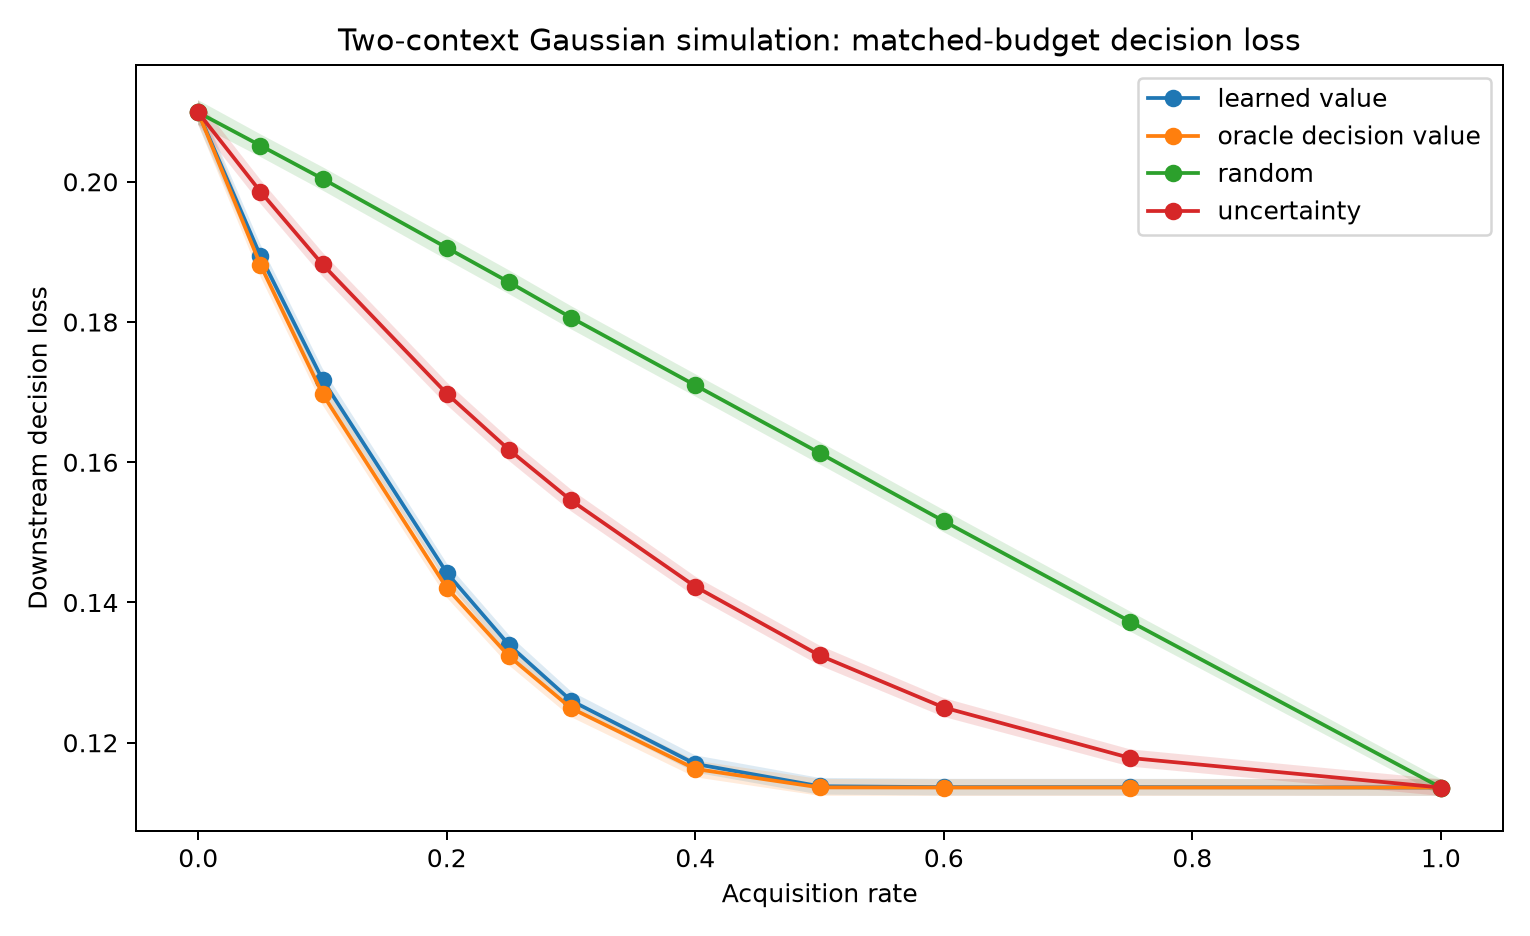
\includegraphics[width=0.82\textwidth]{figures/simulation_matched_budget_decision_loss.png}
\caption{Matched-budget decision loss in the two-context Gaussian experiment. Every policy acquires exactly the same number of optional-monitor outputs at each budget.}
\label{fig:simloss}
\end{figure}

At 25\% acquisition, uncertainty has mean decision loss 0.161797, learned value 0.133958, and oracle value 0.132353. The learned reduction relative to uncertainty is 0.027839 with paired 95\% interval $[0.027368,0.028310]$. At 50\%, learned and oracle losses are 0.113794 and 0.113628, compared with 0.132450 for uncertainty. Mean Spearman correlation between predicted and analytic value is 0.9396.

\begin{figure}[htbp]
\centering
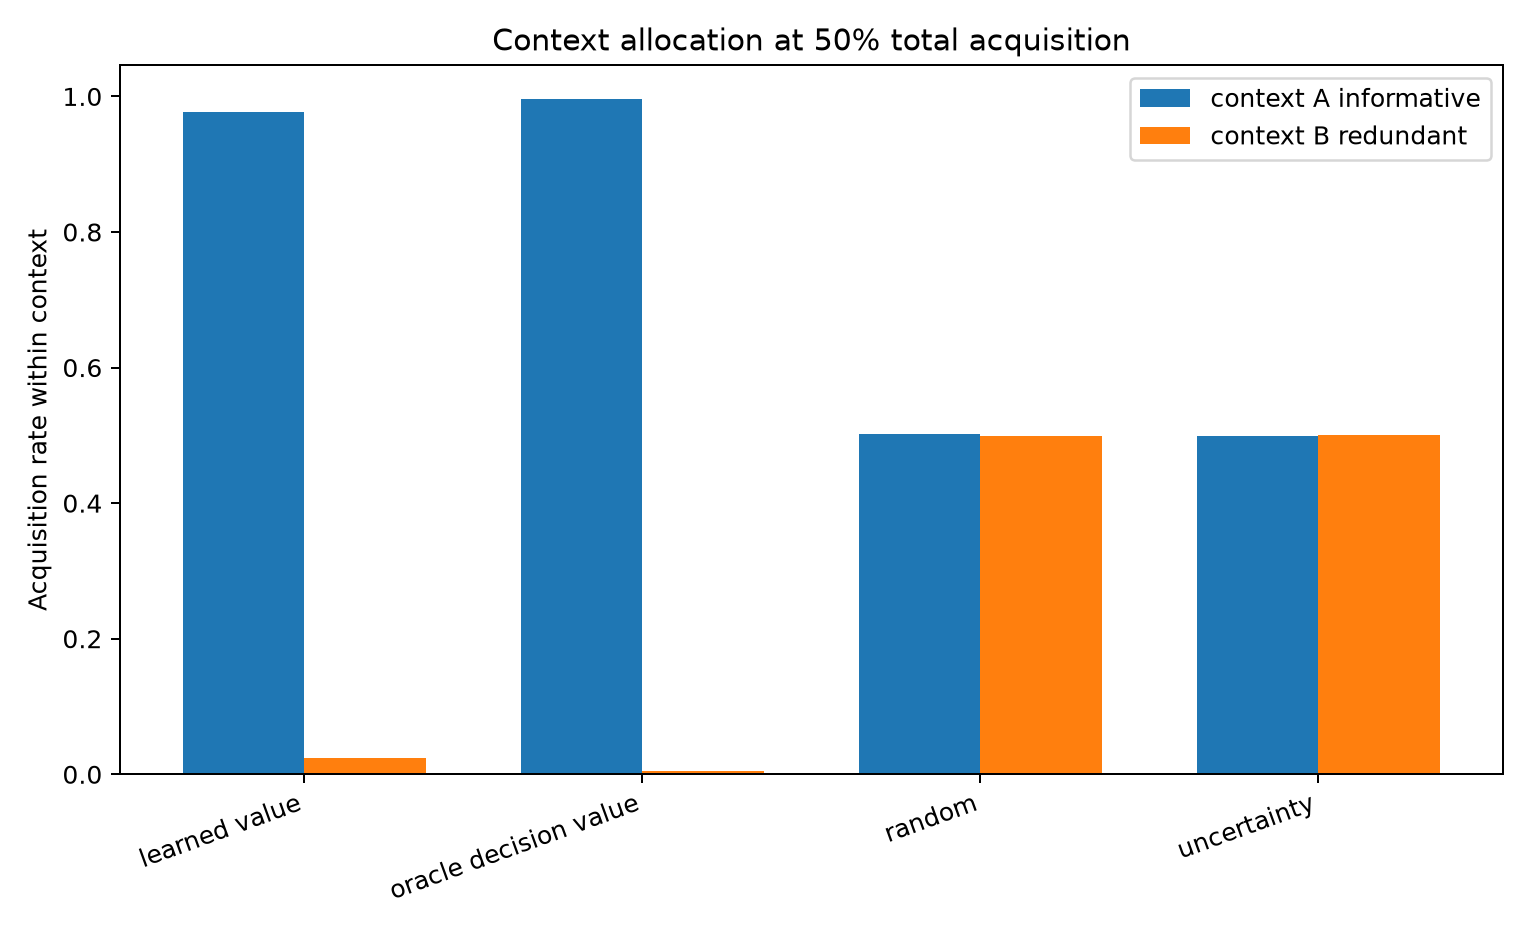
\includegraphics[width=0.77\textwidth]{figures/simulation_context_allocation.png}
\caption{Context allocation at 50\% acquisition. Value-based policies concentrate calls in the informative context, whereas uncertainty cannot use the monitor-quality difference.}
\label{fig:simallocation}
\end{figure}

The simulation validates the requested mechanism under controlled conditions. It is not evidence that the same separation is learnable in the real dataset.

\section{Real-data results}

\subsection{Complementary monitor value}

\Cref{tab:complementarity} summarizes the development-only cross-fitted targets. Acquiring the compact monitor after the rule filter changes only 2.02\% of decisions and reduces decision loss by 0.00356. Qwen after rule and compact changes 18.79\% of decisions and reduces decision loss by 0.10729. It corrects 249 decisions and worsens 68. The Qwen setup therefore satisfies the first milestone condition: at least one heterogeneous monitor has complementary value.

\begin{table}[htbp]
\centering
\caption{Cross-fitted complementary-value diagnostics.}
\label{tab:complementarity}
\begin{tabularx}{\textwidth}{@{}lrrrrrr@{}}
\toprule
Setup & Base loss & Aug. loss & Reduction & $V=1$ & $V=-1$ & Change rate \\
\midrule
Compact after rule & 0.17783 & 0.17427 & 0.00356 & 20 & 14 & 0.02015 \\
Qwen after rule + compact & 0.17487 & 0.06758 & 0.10729 & 249 & 68 & 0.18791 \\
\bottomrule
\end{tabularx}
\end{table}

\begin{figure}[htbp]
\centering
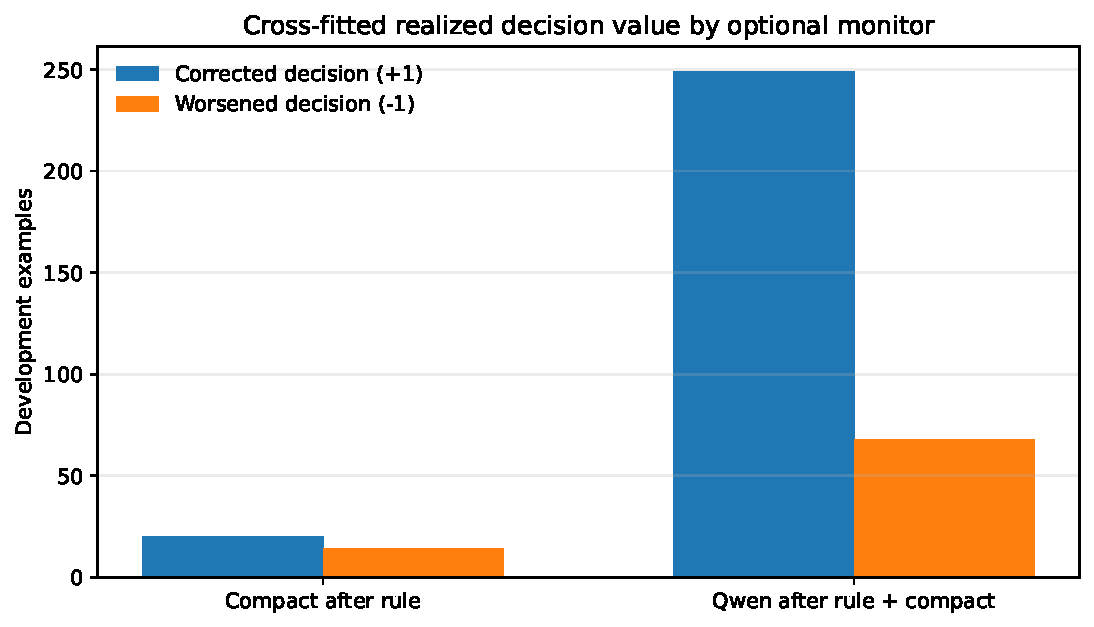
\includegraphics[width=0.76\textwidth]{figures/real_data_complementary_value.pdf}
\caption{Positive and negative realized decision-value counts. Zero-value examples are omitted from the plot: 1,653 for compact acquisition and 1,370 for Qwen acquisition.}
\label{fig:complementarity}
\end{figure}

\subsection{Value predictability: prespecified no-go}

The six-family results are shown in \cref{tab:predictability}. For the primary Qwen/all-features comparison, the pooled outer-OOF Spearman correlation is 0.2529 and positive-value average precision is 0.3619. The integrated learned-minus-uncertainty advantage is positive, 0.004816, but the paired 95\% interval is $[-0.001705,0.011485]$. Because the lower endpoint is not above zero, the prespecified predictability criterion does not pass. None of the 12 setup/family comparisons passes this criterion.

\begin{table}[htbp]
\centering
\caption{Qwen value-predictability results across the six prespecified feature families.}
\label{tab:predictability}
\small
\begin{tabularx}{\textwidth}{@{}Yrrrrr@{}}
\toprule
Feature family & MSE & Spearman & Positive AP & Integrated advantage & 95\% CI \\
\midrule
Cheap features & 0.1693 & 0.2109 & 0.3280 & 0.00062 & $[-0.00559,0.00640]$ \\
Runtime metadata & 0.1720 & 0.2094 & 0.3017 & -0.00037 & $[-0.00751,0.00636]$ \\
Frozen embedding & 0.1793 & 0.1217 & 0.2437 & -0.00943 & $[-0.01789,-0.00114]$ \\
Cheap + metadata & 0.1663 & 0.2443 & 0.3646 & 0.00470 & $[-0.00172,0.01097]$ \\
Cheap + embedding & 0.1670 & 0.2455 & 0.3439 & 0.00525 & $[-0.00101,0.01141]$ \\
All features (primary) & 0.1662 & 0.2529 & 0.3619 & 0.00482 & $[-0.00170,0.01149]$ \\
\bottomrule
\end{tabularx}
\end{table}

\begin{figure}[htbp]
\centering
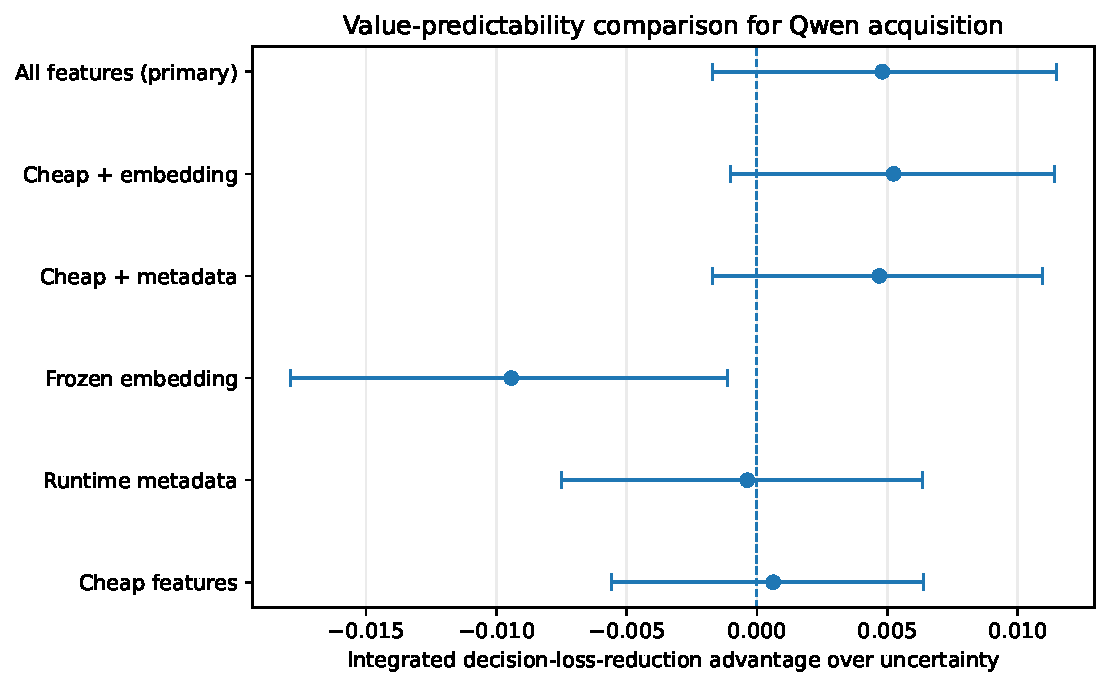
\includegraphics[width=0.82\textwidth]{figures/value_predictability_intervals.pdf}
\caption{Integrated matched-budget advantage over ordinary uncertainty for Qwen acquisition. Error bars are paired 95\% bootstrap intervals. The primary all-features interval crosses zero.}
\label{fig:predictability}
\end{figure}

The positive point estimate is not ignored, but it is not reported as a demonstrated improvement. Repeatedly changing predictors or hyperparameters after seeing this interval would convert the frozen evaluation into exploratory tuning on the same development data.

\subsection{Common-risk safety-cost frontier}

The frontier condition passes. Seven learned points, from 10\% through 75\% requested acquisition, exceed both baselines under the frozen common-risk and common-cost rules. The lowest-cost passing point has actual acquisition rate 0.09781, incremental cost 315.75 ms per example, recall 0.33677, precision 0.71014, and FPR 0.02865. Under the same cost ceiling, the best uncertainty point has recall 0.23368; the random 97.5th-percentile recall is 0.30421.

\begin{table}[htbp]
\centering
\caption{Lowest-cost passing development-only selective point.}
\label{tab:selected}
\begin{tabularx}{\textwidth}{@{}lrrrY@{}}
\toprule
Policy/comparator & Cost (ms/example) & Recall & FPR & Interpretation \\
\midrule
Learned value, 10\% budget & 315.75 & 0.33677 & 0.02865 & Selected point \\
Best uncertainty under cost & 156.25 & 0.23368 & 0.00931 & Lower recall under ceiling \\
Random 97.5th percentile & 156.25 & 0.30421 & -- & Learned recall exceeds upper random baseline \\
\bottomrule
\end{tabularx}
\end{table}

\begin{figure}[htbp]
\centering
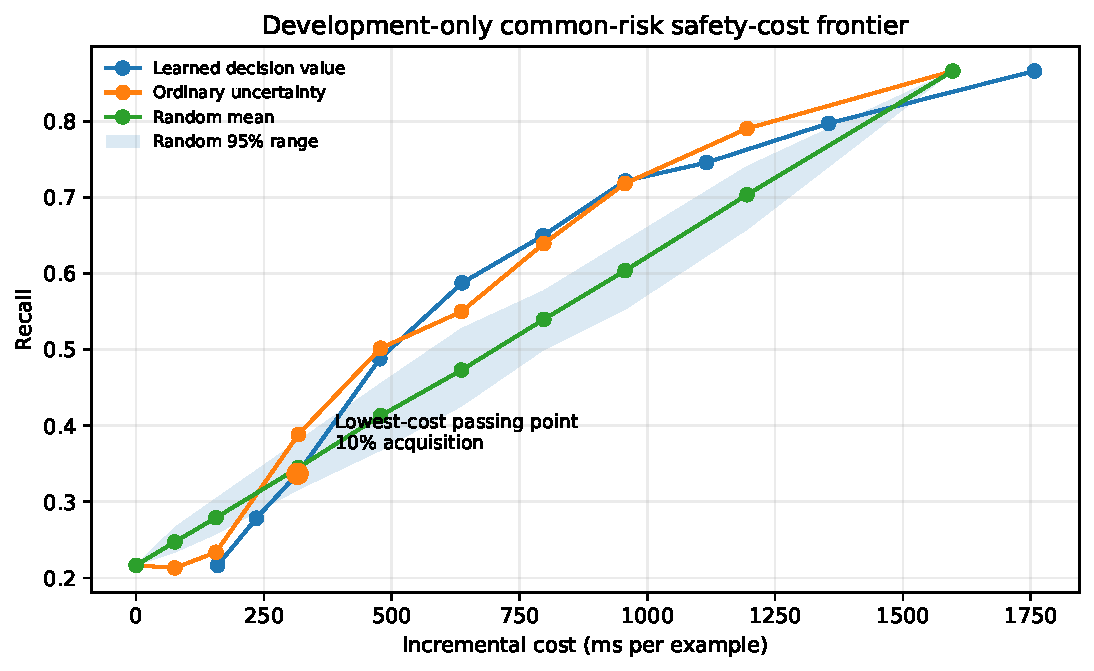
\includegraphics[width=0.83\textwidth]{figures/common_risk_recall_cost_frontier.pdf}
\caption{Recall versus incremental cost for the frozen primary setup. The learned policy includes fixed embedding and value-inference overhead; uncertainty and random do not.}
\label{fig:frontier}
\end{figure}

\begin{figure}[htbp]
\centering
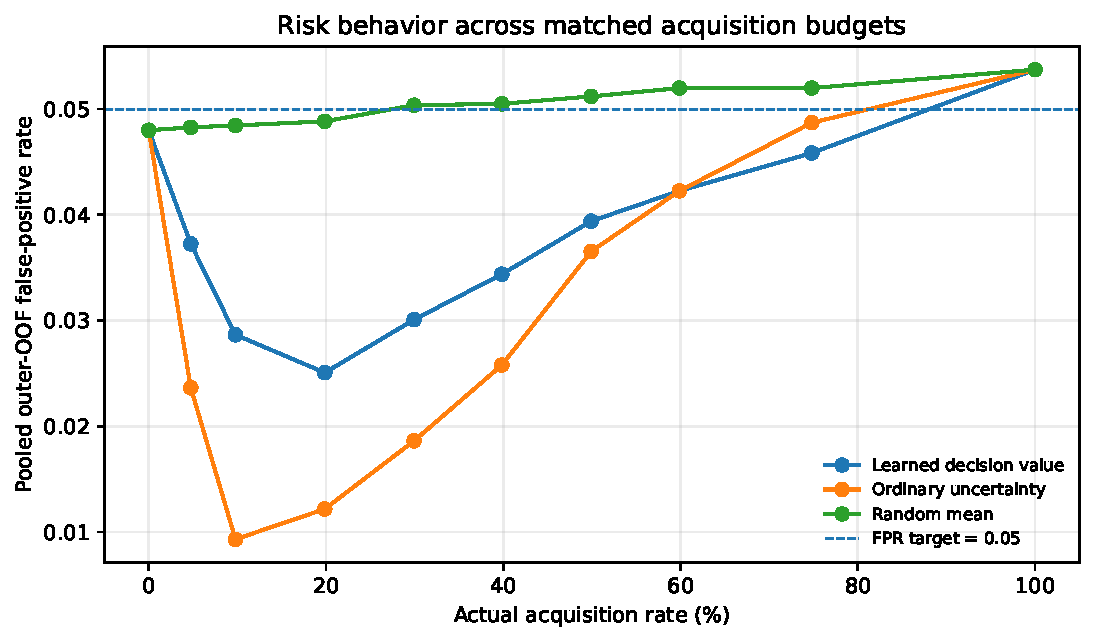
\includegraphics[width=0.83\textwidth]{figures/common_risk_fpr_by_budget.pdf}
\caption{Pooled outer-OOF FPR across matched acquisition rates. Full Qwen acquisition exceeds the empirical 0.05 limit, while all learned points below full acquisition remain feasible in this development diagnostic.}
\label{fig:fpr}
\end{figure}

The frontier pass and predictability no-go are compatible. The frontier asks whether at least one local operating point dominates specified baselines under a cost ceiling and empirical FPR rule. The predictability gate asks whether learned value has a positive integrated advantage across the entire matched-budget curve with a confidence interval excluding zero. The local evidence is useful, but it does not satisfy the broader prespecified gate.

\subsection{Milestone decision}

\begin{table}[htbp]
\centering
\caption{Professor-directed development milestone.}
\label{tab:milestone}
\begin{tabularx}{\textwidth}{@{}>{\raggedright\arraybackslash}p{0.37\textwidth}cY@{}}
\toprule
Condition & Result & Basis \\
\midrule
Heterogeneous monitor has complementary value & \pass & Qwen reduces cross-fitted decision loss by 0.10729. \\
Value is predictably better than uncertainty & \nogo & The primary paired 95\% interval crosses zero. \\
Selective point improves common-risk frontier & \pass & The 10\% point exceeds uncertainty and the random upper baseline. \\
Excluded partitions did not influence result & \pass & Exclusions, fold assignments, and artifact hashes are recorded. \\
\midrule
Overall milestone & \nogo & Every condition was required; no scaling or new-method claim follows. \\
\bottomrule
\end{tabularx}
\end{table}

Since the milestone requires every condition, the project remains no-go. The unused \code{final\_test} and \code{held\_out\_shift} partitions remain unopened for decision-value claims.

\section{Reproducibility and implementation record}

The repository records dataset and model revisions, fold assignments, script hashes, generated artifacts, timing manifests, and strict SHA-256 checks. The complete implementation includes:

\begin{itemize}
  \item 2,159 audited examples and a 95-column monitor-score cache;
  \item exact rule-score regeneration and pinned compact/Qwen model revisions;
  \item 1,687 complete-text frozen embeddings with zero truncation;
  \item 3,374 outer-OOF decision-value target rows;
  \item 13,496 leakage-safe nested value-training rows;
  \item 20,244 outer-OOF value predictions across 2 setups and 6 feature families;
  \item exact matched-budget curves and 100 random repetitions per budget;
  \item measured CPU value-policy inference overhead and GPU optional-monitor costs; and
  \item 39 passing tests at analysis commit \code{788cc51}.
\end{itemize}

The primary verification commands are:
\begin{verbatim}
python scripts/verify_reproducibility.py --strict-hashes
pytest -q
\end{verbatim}
The report is compiled from LaTeX with \code{bash paper/build\_report.sh}.

\section{Discussion}

Three findings are most important. First, monitor complementarity is strong but sparse. Qwen corrects many more decisions than it worsens, yet most examples still have zero realized value. A useful router must identify a relatively small subset without observing the Qwen output itself.

Second, the controlled simulation and real data differ in a revealing way. In the toy experiment, context explicitly identifies whether the optional monitor is informative, and predicted value closely tracks analytic value. In the real dataset, legitimate pre-acquisition features produce positive but uncertain integrated advantage. Complete-text embeddings do not solve the problem by themselves; the embedding-only family is worse than uncertainty for Qwen acquisition. The available representation may encode semantic content without isolating the conditional cases in which Qwen changes the correct decision.

Third, a local common-risk operating point can pass even when the integrated predictability criterion fails. At 10\% acquisition, the learned ranking places enough high-value examples near the top to improve recall under the frozen cost rule. Performance elsewhere on the curve is not uniformly strong enough to make the integrated paired interval positive. Reporting both results avoids reducing the study to either an overly negative or overly favorable summary.

The earlier threshold router remains relevant as historical context. It demonstrated mean-latency savings, but its risk behavior did not support a stable deployment interpretation. The decision-value pivot improves the scientific target: acquisition should be judged by expected downstream benefit, not uncertainty alone. It does not, on this evidence, establish that the benefit is reliably learnable from the current development data.

\section{Limitations}

\begin{itemize}
  \item The real-data evaluation is development-only. No confirmatory decision-value result is reported on \code{final\_test} or \code{held\_out\_shift}.
  \item The dataset combines three public sources and is not representative of all deployment traffic or safety policies.
  \item Labels were audited by one author. Inter-annotator agreement is unavailable.
  \item Realized value is defined through zero-one downstream decisions at thresholds chosen for empirical FPR 0.05. Other losses or policy costs could change the value target.
  \item Positive and negative value events are imbalanced and sparse, especially for compact acquisition.
  \item The complete-text embedding is general-purpose. No representation was trained specifically to predict monitor complementarity.
  \item Cost accounting combines a Tesla T4 Qwen benchmark with CPU embedding and value-inference measurements. It is a documented incremental comparison, not a single-hardware end-to-end benchmark for the new policy.
  \item Random-baseline intervals describe the 100 frozen repetitions; they are not population confidence guarantees.
  \item The common-risk frontier uses empirical pooled outer-OOF FPR, not a new finite-sample certificate for the learned acquisition policy.
  \item The study does not model correlated monitor failures, arbitrary distribution shift, online adaptation, or adversarial adaptation to the router.
  \item The no-go outcome should not be reversed by post-hoc retuning on the same development folds. Any extension requires a separately frozen protocol and fresh confirmatory evidence.
\end{itemize}

\section{Conclusion}

Decision value is the appropriate target for optional safety-monitor acquisition: a monitor should be called when its expected reduction in downstream decision loss exceeds its cost. The counterexample and Gaussian experiment establish why uncertainty alone can be suboptimal. The real-data analysis confirms that Qwen has substantial complementary value and identifies development-only selective points with favorable recall, FPR, and measured incremental cost.

The stronger required claim does not pass. The primary learned-value ranking has positive integrated advantage over uncertainty, but the paired 95\% confidence interval includes zero. The overall milestone is therefore no-go, and the study does not claim a new validated routing method, shift robustness, or deployment readiness.

The completed work provides a reproducible measurement framework for future investigation: monitor-specific value targets, nested leakage controls, complete-text representations, exact matched budgets, and common-risk cost accounting. A future extension should be separately preregistered and evaluated on fresh data rather than tuned against the completed diagnostic.

\appendix
\section{Detailed compact-monitor feature-family results}

\begin{table}[htbp]
\centering
\caption{Compact-after-rule value-predictability results.}
\small
\begin{tabularx}{\textwidth}{@{}Yrrrrr@{}}
\toprule
Feature family & MSE & Spearman & Positive AP & Integrated advantage & 95\% CI \\
\midrule
Cheap features & 0.01862 & 0.06628 & 0.36317 & -0.00056 & $[-0.00280,0.00153]$ \\
Runtime metadata & 0.02108 & 0.03231 & 0.04917 & -0.00199 & $[-0.00488,0.00093]$ \\
Frozen embedding & 0.02126 & 0.01922 & 0.01962 & -0.00231 & $[-0.00550,0.00093]$ \\
Cheap + metadata & 0.01908 & 0.07485 & 0.26492 & 0.00006 & $[-0.00222,0.00237]$ \\
Cheap + embedding & 0.01971 & 0.10347 & 0.23068 & 0.00096 & $[-0.00132,0.00336]$ \\
All features & 0.01946 & 0.08381 & 0.24795 & 0.00012 & $[-0.00209,0.00213]$ \\
\bottomrule
\end{tabularx}
\end{table}

\section{Primary learned-policy frontier points}

\begin{longtable}{@{}rrrrrr@{}}
\caption{Primary learned-value points on the development frontier.}\label{tab:allfrontier}\\
\toprule
Budget & Actual rate & Cost (ms) & Recall & FPR & Decision loss \\
\midrule
\endfirsthead
\toprule
Budget & Actual rate & Cost (ms) & Recall & FPR & Decision loss \\
\midrule
\endhead
0.00 & 0.0000 & 159.50 & 0.2165 & 0.0480 & 0.1749 \\
0.05 & 0.0474 & 235.26 & 0.2784 & 0.0372 & 0.1553 \\
0.10 & 0.0978 & 315.75 & 0.3368 & 0.0287 & 0.1381 \\
0.20 & 0.1986 & 476.74 & 0.4880 & 0.0251 & 0.1091 \\
0.30 & 0.2993 & 637.72 & 0.5876 & 0.0301 & 0.0960 \\
0.40 & 0.3983 & 795.87 & 0.6495 & 0.0344 & 0.0889 \\
0.50 & 0.4991 & 956.86 & 0.7216 & 0.0394 & 0.0806 \\
0.60 & 0.5987 & 1115.95 & 0.7457 & 0.0423 & 0.0788 \\
0.75 & 0.7481 & 1354.59 & 0.7973 & 0.0458 & 0.0729 \\
1.00 & 1.0000 & 1757.06 & 0.8660 & 0.0537 & 0.0676 \\
\bottomrule
\end{longtable}

\section{Key repository artifacts}

\begin{description}[style=nextline,leftmargin=0pt,labelindent=0pt,font=\normalfont\ttfamily]
\item[\path{configs/decision_value_real_data_protocol_v1.json}]
Frozen development-only protocol, feature families, budgets, and milestone rules.
\item[\path{paper/decision_value_theory.tex}]
Formal derivation and counterexample source.
\item[\path{reports/decision_value_gaussian_simulation/}]
Seed-level simulation results, matched-budget tables, and figures.
\item[\path{reports/decision_value_real_data/cross_fitted_decision_value_targets.csv}]
Outer-OOF complementarity targets.
\item[\path{reports/decision_value_real_data/nested_value_training_targets.csv}]
Leakage-safe value-estimator training targets.
\item[\path{reports/decision_value_real_data/value_predictability_summary.csv}]
Six-family matched-budget predictability results.
\item[\path{reports/decision_value_real_data/common_risk_safety_cost_frontier.csv}]
Deterministic learned and uncertainty frontier.
\item[\path{data/metadata/reproducibility_manifest.json}]
Strict file hashes and final decision summaries.
\end{description}

\begingroup
\small
\setlength{\bibitemsep}{0.35\baselineskip}
\printbibliography
\endgroup

\end{document}
